%This is the first chapter of the dissertation

%The following command starts your chapter. If you want different titles used in your ToC and at the top of the page throughout the chapter, you can specify those values here. Since Columbia doesn't want extra information in the headers and footers, the "Top of Page Title" value won't actually appear.
%\makepagestyle{cu}
%\copypagestyle{cu}{ruled}
%	\makeevenfoot{cu}{}{\thepage}{}
%	\makeoddfoot{cu}{}{\thepage}{}

\pagestyle{cu}
\graphicspath{{./Chapter1/images/}}

\chapter[Dark Matter][Dark Matter]{Dark Matter}

For nearly a century, experimental evidence has suggested that a large portion of the universe is made up of a non-luminous type of matter.  While this dark matter has only been detected indirectly via its interaction with normal matter through the gravitational force, recent experiments conclude that approximately 26\% of the entire energy density of the universe is comprised by dark matter.

	In this chapter, I will focus on the leading dark matter model, the experimental evidence for its existence, the different candidates for particle dark matter, and the current detection methods employed in the search for particle dark matter.
	
	
\section{$\boldsymbol{\Lambda}$CDM Model}
\label{sec:cdm}

	One of the guiding principles of cosmology are the assumptions that the universe is both homogeneous and isotropic at large enoug scales (typically on the order 100 Mpc or $10^{5}$ light years).  Continuing with these principles and maintaining generality, we can arrive at the Robertson-Walker space-time metric
	\begin{equation}
		ds = -c^{2}dt^{2} + a(t)^{2}\left( \dfrac{dr^{2}}{1 - kr^{2}} + r^{2}d\Omega^{2}\right)
	\end{equation}
Here, $a(t)$ is called the \emph{scale factor}, an arbitrary function of time allowing for time dependent changes of the universe, and $k$ is a constant modeling the curvature of the universe.  For $k=-1$, the universe is considered open, for $k=1$, the universe is considered close, and at $k=0$ we are left with our Euclidean (flat) universe.  Note that for $a(t) = 1$ and $k = 0$ the Robertson-Walker metric reduces to the Minkowski metric.

	Using this metric in combination with Einstein's equation we can derive the equations for the Friedmann-Robertson-Walker universe described by the Friedmann equations.
	
	\begin{equation}
		\frac{\ddot{a}}{a} = -\frac{4 \pi G}{3} \left( \rho + 3p \right)
	\end{equation}
	\begin{equation}
		\left( \frac{\dot{a}}{a}\right)^{2} = \frac{8 \pi G}{3} \rho - \frac{k}{a^2}
	\end{equation}

	We can define several useful (and commonplace) parameters to simplify the second Friedmann equation further.
\\
\\
\textbf{Hubble Parameter}: $ H = \frac{\dot{a}}{a} $\\
\textbf{Critical Density}: $ \rho_{crit} = \frac{3H^2}{8 \pi G} $\\
\textbf{Density Parameters}: $ \Omega_{i} = \frac{8 \pi G}{3H^2}$,  $\Omega_{i} = \frac{\rho_{i}}{\rho_{crit}} $\\
\begin{equation}
	\Omega - 1 = \frac{k}{H^2 a^2}, \ \ \ \ \Omega = \sum_{i} \Omega_{i} = \Omega_{\Lambda} + \Omega_{CDM} + \Omega_{Baryon} + \Omega_{Rad}  \ldots 
\end{equation}
	
	Here the critical density is defined such that the universe is flat ($k=0$).  One can think of $\frac{\Omega_i}{\Omega}$ as what part of the total matter and energy budget a particular component makes up.  The main contributors to the density of the universe are dark energy and cold dark matter hence the $\Lambda$CDM Model.  Measurements of the various density parameters and other $\Lambda$CDM parameters has been a very big area of research over the last two decades and will be discussed later in this chapter.
	
\section{Evidence of Dark Matter}

\subsection{Dynamical Constraints from Clusters of Galaxies}

The first evidence of dark matter came from Fritz Zwicky in 1933.  Zwicky used a basic application of the virial theorem on galaxies in the Coma Cluster	to estimate the mass of the cluster.  He then  estimated the total mass based on the brightness of the cluster and found significant disagreement between the results leading him to the conclusion that ``if this would be confirmed we would get the surprising result that dark matter is present in much greater amount than luminous matter.'' \cite{Zwicky1933}
	
\begin{figure}[h]
\includegraphics[width=8cm]{coma_composite}
\centering
\caption{A composite image combining an X-ray data, courtesy of Chandra, and optical data, courtesy of the Sloan Digital Sky Survey.  Image credit: X-ray - NASA/CXC/MPE/J.Sanders et al, Optical - SDSS}
\end{figure}
	
	
\subsection{Dynamical Constraints from Galactic Rotation Curves}	
	
%\href{http://www.skyandtelescope.com/astronomy-resources/vera-rubin-dark-matter-detective/}{summary source}	

%\href{http://articles.adsabs.harvard.edu/full/1970ApJ...159..379R}{rubin paper source}	

\begin{figure}[b]
	\centering
	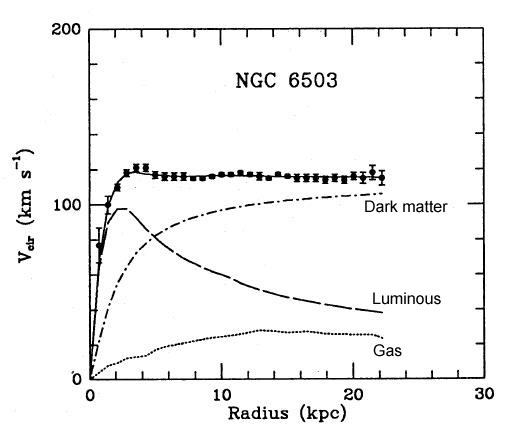
\includegraphics[width=8cm]{ngc_6503_rotation_curve}
	\caption{The rotation curve of the galaxy NGC 6503 broken down into individual components: visible matter (dashed), gas (dotted), and dark matter (dash dotted) \cite{Begeman1991}. }
	\label{fig:galactic_rotation_curve}
\end{figure}

	
Nearly fourty years later, stronger evidence was provided for the existence of dark matter by Vera Rubin and Kent Ford in their 1970 paper looking at the rotation curve of the Andomeda Galaxy \cite{rubin1970rotation}.  In this paper, Rubin used the H$\alpha$ lines to determine the orbital velocities of different stars in the galaxy.  Later measurements used the 21 cm hyperfine transition line to measure orbital velocities within other galaxies \cite{Begeman1991}.
	
	From simple Newtonian arguments, one gets the following description of the orbital velocity inside a galaxy:
	
\begin{equation}
v(r) = \sqrt{\frac{G M(r)}{r}}
\end{equation}	

In this equation, M(r) is the sum of the masses of all the gas and stars inside a given radius.  Given that most of the mass from luminous matter is concentrated at the center, one would expect that at large distances from the center of the galaxy, the orbital velocity would fall off as $v \propto r^{-1/2}$.

However, what is seen differs from this simple approximation drastically.  \figref{fig:galactic_rotation_curve} is taken from \citeref{Begeman1991} but the results are similar to what Rubin and Ford saw deecades earlier: the asymptotic behavior of the orbital velocity is constant and does not show any polynomial roll-off.  By isolating the contributions from measurable mass densities (such as visible matter and gas), one can get an idea of the density distribution of dark matter in a galaxy.  From the figure below, one could asymtotically estimate that $M(r) \propto r$ which would imply that $\rho(r) \propto r^{-2}$.  One quickly realizes that this cannot be the true density since the mass of the galaxy diverges but approximates the density within an effective radius.



\subsection{Evidence from Graviational Lensing}	

Gravitational lensing is the distortion of light coming from a source due to the warping of spacetime from the presence of large amounts of matter or energy.  This effect is illustrated in \figref{fig:gravitation_lensing_cartoon} and actually captured in the form of an Einstein Cross in \figref{fig:einstein_cross}.  In a gravitational lensing system, if we know the redshift (distance) of the source and the lense, we can estimate the gravitational field of the lensing system and hence its mass.


\begin{figure}[t]
	\centering
	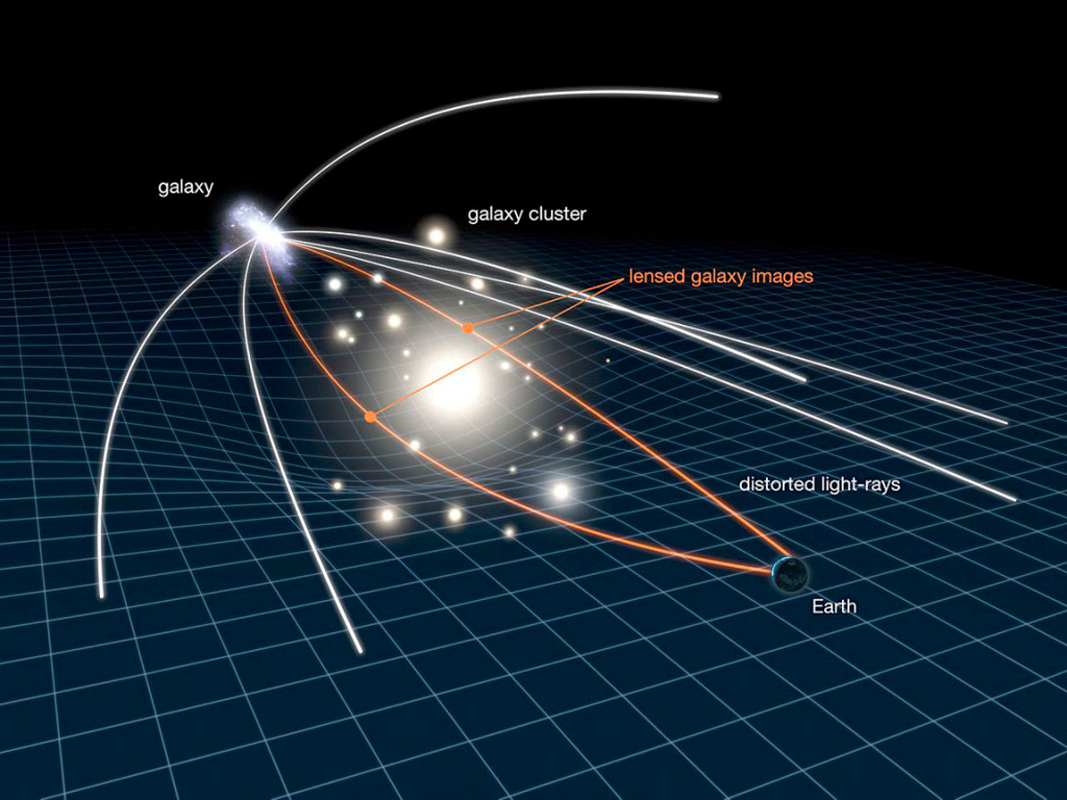
\includegraphics[width=0.8\textwidth]{gravitation_lensing_cartoon}
	\caption{A cartoon showing the deflection of light due to the warping of spacetime caused by the presence of a massive galaxy cluster.  Note that for very strong lensing, one expects multiple images of the source object and sometimes even an Einstein Ring around the lense. Image credit: NASA/ESA.}
	\label{fig:gravitation_lensing_cartoon}
\end{figure}

\begin{figure}[t]
	\centering
	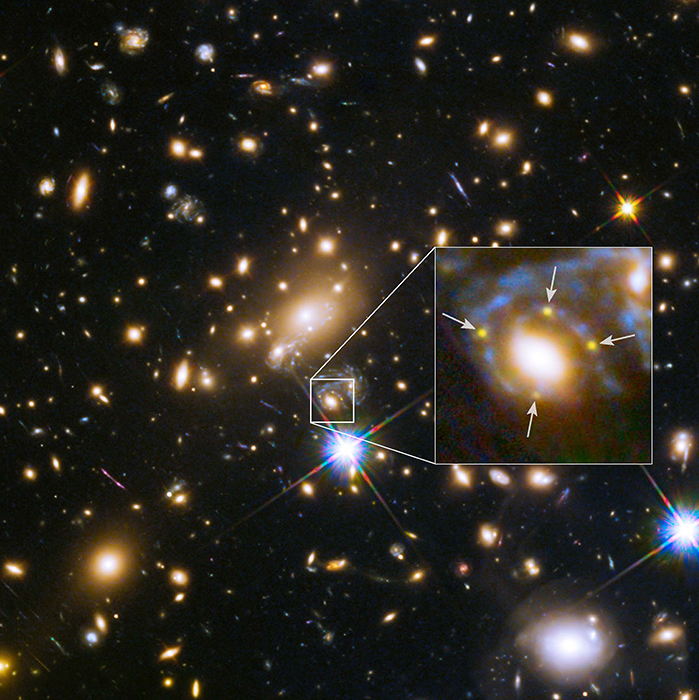
\includegraphics[width=0.8\textwidth]{einstein_cross}
	\caption{In this optical image you see the massive MACS J1149.6+2223 cluster.  In the zoomed portion, you can actually see the same supernova, SN Refsdal, in four smaller images around a large galaxy within the cluster. Image credit: HST.}
	\label{fig:einstein_cross}
\end{figure}


%\begin{SCfigure}[\sidecaptionrelwidth][h]
%	\centering
%	\caption{In this optical image you see the massive MACS J1149.6+2223 cluster.  In the zoomed portion, you can actually see the same supernova, SN Refsdal, in four smaller images around a large galaxy within the cluster. Image credit: HST.}
%	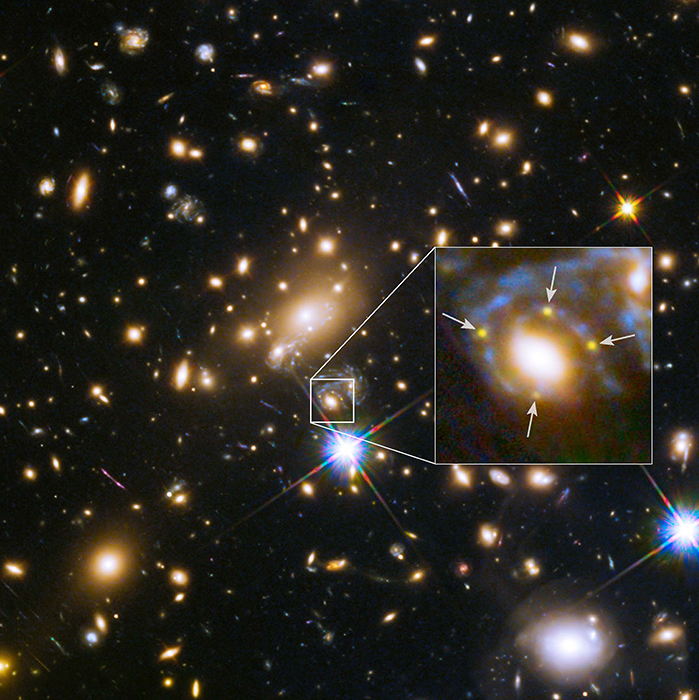
\includegraphics[width=0.5\textwidth]{einstein_cross}
%\end{SCfigure}

Mass estimation via gravitational lensing in itself is very useful for finding large discrepancies in mass from known sources and true mass (the discrepancy being attributed to dark matter).  However, when combined with x-ray measurements, as seen in \figref{fig:bullet_cluster}, one gets even more interesting results.  Shown in \figref{fig:bullet_cluster} is the Bullet Cluster (1E0657-558) which actually consists of two colliding sub-clusters.  In the image on the left, one can see the infrared image from Magellan that is used, along with optical images from Hubble, to estimate the mass distribution of each galaxy cluster through graviational lensing.  In the right image, one can see the X-ray map of the Bullet Cluster from the Chandra X-ray observatory with the same mass contours: one can see that the plasma from the clusters interacts giving the cone shapes in the center.  However, the mass contours largely remained centered on the individual clusters (as seen in the optical image) implying that the majority of the matter interacted minimally during the collision \cite{clowe2006direct}.  This implies that the majority of the matter in these clusters at least does not interact electromagnetically.

% https://astrobites.org/2016/11/04/the-bullet-cluster-a-smoking-gun-for-dark-matter/

\begin{figure}[t]
	\centering
	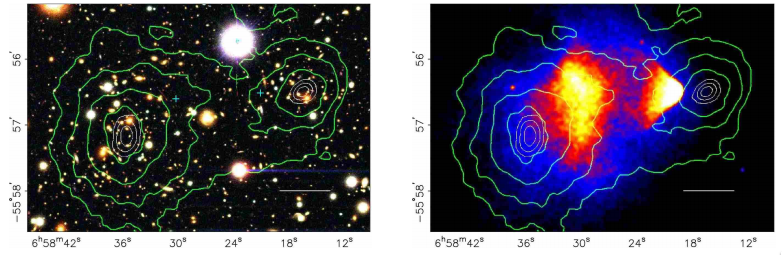
\includegraphics[width=0.999\textwidth]{bullet_cluster}
	\caption{Infrared (left) and X-ray (right) maps of the Bullet Cluster (1E0657-558).  While the plasma in the clusters interacts during the collision of the two individual clusters, as is seen by the shockwave in the center, the majority of the mass passes right through \cite{clowe2006direct}.}
	\label{fig:bullet_cluster}
\end{figure}


\subsection{Evidence from the Cosmic Microwave Background}

The Cosmic Microwave Background (CMB) has proved to be one of the richest discoveries in all of cosmology.  Accidentally discovered in 1964 by Penzias and Wilson \cite{penzias1965measurement}, the radiation from the CMB is almost perfectly isotropic and described by a blackbody spectrum at 2.725 K \cite{fixsen1996cosmic}.  The isotropy in the CMB provides the strongest evidence to date of the Big Bang Hypothesis and helped to formulate our current picture of the early universe down to the recombination epoch, where the universe was sufficiently cool such that hydrogen could form from the free electrons and protons in turn allowing photons to travel freely through the universe.  

\begin{figure}[ht]
	\centering
	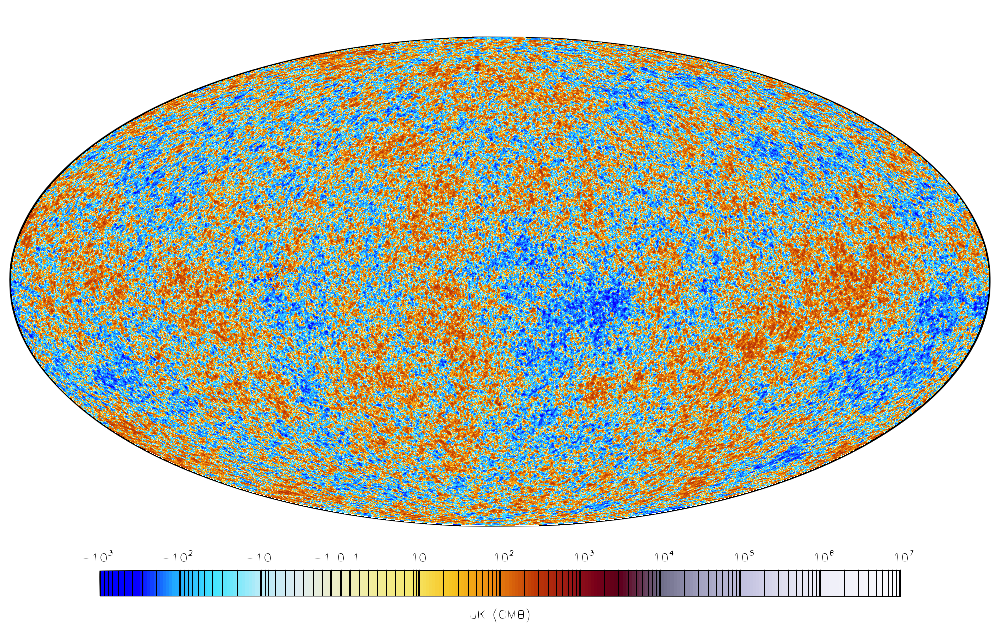
\includegraphics[width=0.95\textwidth]{planck_map}
	\caption{The Planck 2015 measurement of the temperature anisotropy of the CMB.  Note that the largest deviations from the mean are on the order of $200 \mu K$ from the 2.725 K mean (roughly 1 in $10^4$).  Image credit: IRSA, \cite{Ade2015}.}
	\label{fig:planck_map}
\end{figure}

\begin{figure}[ht]
	\centering
	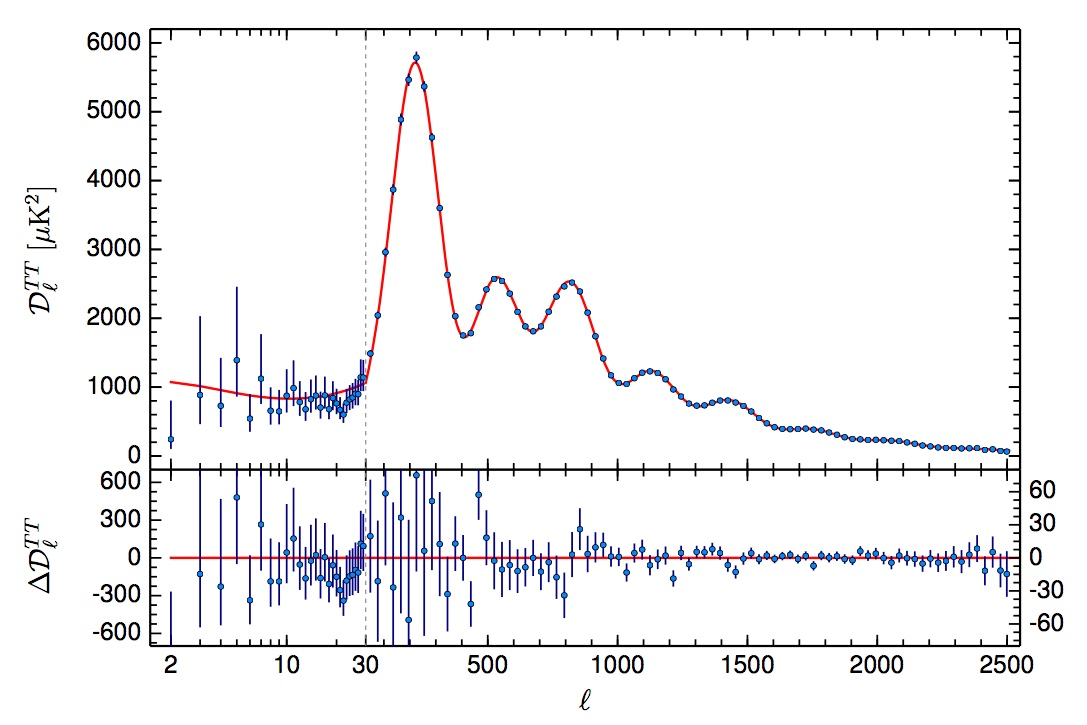
\includegraphics[width=0.95\textwidth]{planck_2015_power_spectrum}
	\caption{The power spectrum of the temperature anisotropies measured by Planck along with the best fit prediction from the $\Lambda$CDM model.  $\mathcal{D}_l^{TT}$ is a proxy for $C_i$ and is defined $\mathcal{D}_l^{TT} \equiv l(l+1)C_l / 2 \pi$ \cite{Ade2015}.}
	\label{fig:planck_fit}
\end{figure}

% https://www.astro.umd.edu/~miller/teaching/astr422/lecture21.pdf
% http://w.astro.berkeley.edu/~mwhite/rosetta/node2.html

As the CMB has been studied in more detail, cosmologists began to see that there are in fact very small temperature fluctuations on the order of ${\lesssim}100 \mu K$ \cite{bennett1996four, komatsu2011seven, Ade2015}.  These temperature fluctuations, as seen in the 2015 measurement of the CMB by Planck satellite, are shown in \figref{fig:planck_map}.  To characterize the temperature fluctuations of the entire sky, we use the spherical harmonics, $Y_{lm}(\theta, \phi)$.  


\begin{equation}
	T(\theta, \phi) = \sum_{l=0}^{\infty} \sum_{m=-l}^{l} a_{lm} Y_{lm}(\theta, \phi)
\end{equation}

We assume that  the distribution of $a_{lm}$ should be described by a Gaussian distribution, as predicted by inflation, with a mean of 2.725 K for any given multipole moment $l$.  Therefore, the only piece missing to completely describe these $a_{lm}$ for each multiple moment is the variance of  this distribution so we define $C_l \equiv \left<| a_{lm}|^2\right>$.  These $C_l$ form the power spectrum of the CMB and can be used to test various formation models of the universe.  Planck tested the $\Lambda$CDM model described in \secref{sec:cdm} against their power spectrum (\figref{fig:planck_fit}) and found remarkable agreement between prediction and data while constraining some of the universal constants including $H_0$, $\Omega_{\Lambda}$, $\Omega_{CDM}$, $\Omega_{Baryon}$, and $\Omega_{Rad}$.  It is from this fit that we find that our universe has a curvature very close to zero and therefore is flat and that our universe is comprised of roughly  $~68.3\%$ dark energy, $~26.8\%$ dark matter, and $~4.9\%$ ordinary matter \cite{Ade2015}.

The $\Lambda$CDM model has been tested since its inception using N-body simulations to propagate the formation of large scale structure in the universe.  While small discrepancies between simulation and observation have been found, it is clear from these simulations that without cold dark matter it is extremely difficult to explain the large scale structure we see in the universe given the anisotropies of the CMB \cite{navarro1996structure, springel2006large, vogelsberger2014introducing}.



\section{Dark Matter Candidates}
\label{sec:dm_candidates}

While there is an abundance of evidence to suggest that dark matter exists, we have little evidence to suggest what this cold dark matter actually is.  In this section, we will discuss two of the most popular candidates for dark matter and their physical motivations.  It should be noted that the candidates discussed do not form an exhaustive list but do satisfy the most basic requirements of a dark matter candidate:

\begin{itemize}
        \item The lifetime of the particle is much greater than the lifetime of the universe (or is stable)
        \item  The particle must be electrically neutral and very weakly interacting with ordinary matter
        \item The particle must be able to provide the correct relic density of cold dark matter as predicted by the CMB
\end{itemize}


\subsection{Axions}



Axions are hypothetical standard model particles that are introduced via the Peccei-Quinn mechanism as a solution to the strong-CP problem, one of the largest remaining deficiencies in the standard model \cite{axion_1977}.  CP (charge and parity) symmetry violation is required to explain the imbalance of matter and antimatter in the universe (why more matter exists) and has been observed in electroweak theory in a wide variety of measurements \cite{alavi1999observation, fanti1999new, aubert2001measurement, abe2001observation, aaij2013first}.  CP violation has never been observed in quantum chromodynamics even though there are natural terms in the QCD Lagrangian that would allow it.  Therefore, this term in the Lagrangian, must be fine-tuned to exactly zero, hence the strong-CP problem.  The axion introduced by Peccei-Quinn theory replaces this term with a field and gives the Lagrangian natural CP symmetry.

While the discovery of the axion would solve one of the largest problems of standard model, it also has the potential to solve one of the largest open mysteries of cosmology by making up at least a part of the cold dark matter density of the universe.  Even though the axion is expected to have a very small mass ($10^{-6}-10^{-2} eV$) it could still be produced cosmologically such that the large scale structure that we observe in the universe today is explained and we arrive at the CDM density estimated by Planck \cite{graham2015experimental}.

    There are a number of experiments that can provide information about axions, both directly and indirectly.  The mass range of axions, is essentially restricted from cosmological evidence from the CMB and stellar evolution.  Simultaneously, cavity microwave experiments such as ADMX \cite{stern2016admx} and NMR based searches such as CASPeR \cite{garcon2017searching} try to directly detect these low mass CDM candidates.

\begin{figure}[t]
	\centering
	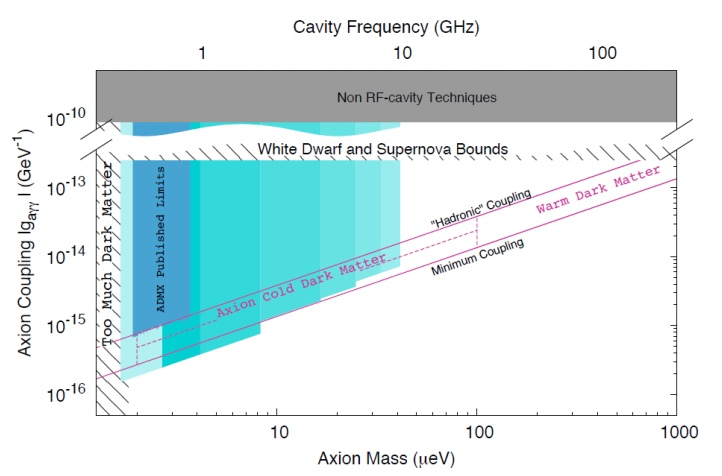
\includegraphics[width=0.95\textwidth]{admx2_limits}
	\caption{The projected sensitivity of the ADMX Generation 2 axion search.  Note that strong cosmological constraints are placed on the mass range and the axion coupling is also constrained by the mass.  The ADMX collaboration predicts that the searches shown will be completed by 2022 \cite{stern2016admx}.}
\end{figure}

\subsection{WIMPs}


Weakly interacting massive particles (WIMPs), which will be the focus of the remainder of this work, have proven to be the most popular dark matter candidate historically.   WIMPs not only satisfy the basic criteria listed at the beginning of this section but additionally they have what is referred to as the ``WIMP Miracle" in their favor.  In the early stages of the universe, the temperature and density were so large that all particles were in a state of chemical equilibrium.  A dark matter particle could annihilate by colliding with its anti-partner to form any type of particle vice versa.  As time passed, however, the universe expanded and cooled making it more unlikely for these dark matter particles to be created or destroyed.  Using this thermal equilibrium model alongside the $\Lambda$CDM model, one can infer that the CDM density in the universe today is approximately given by \cite{jungman1996supersymmetric, bertone2010particle}

\begin{equation}
        \Omega_{CDM}h^2 \approx \frac{3 \times 10^{-27} \mathrm{cm}^3  \mathrm{s}^{-1}}{\left< \sigma_{ann} v \right> }
\end{equation}

where $\left< \sigma_{ann} v \right>$ is thermally averaged annihilation cross-section of cold dark matter.  Incredibly enough, if we assume that cold dark matter has properties such as cross-section and mass on the weak scale, we find that $\Omega_{CDM}h^2 \approx 0.1$, which is in agreement with cosmological constraints. 

In addition to WIMPs agreeing with cosmological evidence, several WIMP-like particles having masses on the order of 100 GeV with very long lifetimes naturally fall out of extensions of the standard model, such as supersymmetry.  



\section{Detecting WIMPs}

\begin{figure}[b]
	\centering
	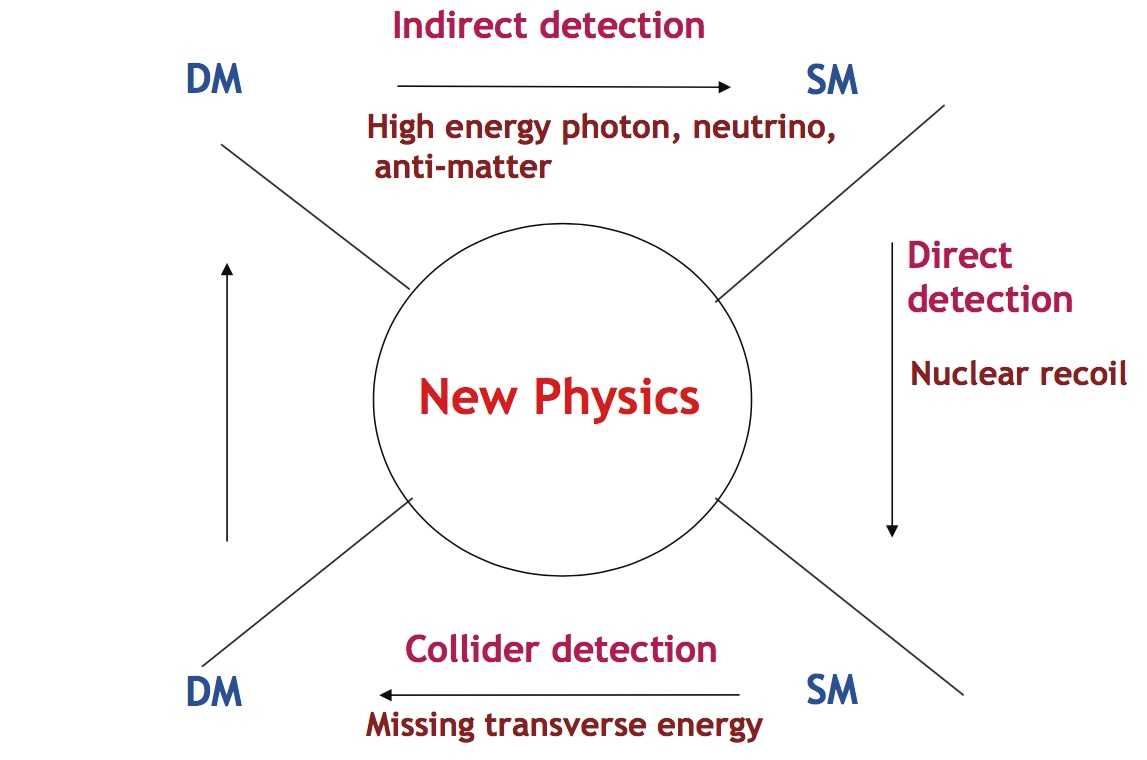
\includegraphics[width=0.75\textwidth]{wimp_detection}
	\caption{The three general approaches to WIMP detection: indirect detection, collider detection, and direct detection.  Image credit: \cite{bi2013status}.}
	\label{fig:wimp_detection}
\end{figure}

Over the last few decades there has been an enormous concerted effort to detect WIMPs.  This effort has been focused in three general approaches: indirect detection, collider detection, and direct detection.  \figref{fig:wimp_detection} shows the idea behind these approaches:

\begin{itemize}
        \item Direct detection looks for the scattering of WIMPs with ordinary matter
        \item Indirect detection looks for the annihilation of WIMPs in our galaxy into ordinary matter
        \item Collider detection is an attempt at creating WIMPs by colliding ordinary matter
\end{itemize}


\subsection{Indirect Detection}

%https://arxiv.org/pdf/1404.1938.pdf

As we know from previous sections, WIMPs, if they make up all (or some) of the dark matter in the universe, must reside in galaxies to explain the odd behavior of rotation curves and the mass discrepancies.  Given the observational evidence, simulations have been created that can predict both the distribution of dark matter within our own and other galaxies \cite{stadel2009quantifying, maccio2007concentration} and the density of dark matter in our own solar system (roughly $0.2 - 0.4$ GeV \cite{read2014local}).  Indirect detection experiments look at high density regions of dark matter halos, such as in or around the Milky Way center and dwarf galaxies, to search for annihilations of WIMPs into detectable particles.

The goal of indirect detection is to capture a dark matter annihilation by observing its byproducts.  In the ideal case, two dark matter particles would annihilate and create two protons with energies equal to the mass of the dark matter particle.  Even though this would be the ``smoking gun" evidence of dark matter, most of the standard model extension WIMPs predict that this would be highly suppressed.  Instead, these indirect experiments are more likely to observe the annihilation of WIMPs into other particles which in turn will produce photons \cite{bi2013status}.  

A major difficulty in indirect detection experiments is distinguishing potential signals from normal astrophysical processes.  Since areas of high dark matter density are also typically areas of high astrophysical activity it becomes difficult to separate potential dark matter signals from potentially new astrophysics \cite{zitzer2015search}.  However, in recent years, astrophysicists have started turning their telescopes towards dwarf galaxies, which are dark matter dominated but have negligible astrophysical backgrounds \cite{conrad2014indirect}.  %For example, in 2012 the Fermi Large Area Telescope (Fermi-LAT) observed a line at 130 GeV near the galatic center in excess of the expected background with a significance of 4.5 sigma \cite{tempel2012fermi}.  However, over the last few years, this line has largely been ruled out by other experiments \cite{abdalla2016hess}



\subsection{Collider Detection}

The main idea behind collider detection is that since the WIMP is expected to have a mass on the order of $1-10^3$ GeV is that we can create it in particle accelerators.  Of course, detectors at particle accelerators are not designed to detect dark matter directly so when searching for WIMPs physicists must actually search for missing transverse energy (MET) in a collision. detect it via the missing transverse energy (MET).  The MET can be reconstructed by observing the outgoing particles and jets in a collision based on momentum conservation.  This reconstruction is shown in \figref{fig:collider_detection}.  Ultimately, this MET can be used to determine the mass and the new physics processes of the WIMP \cite{bi2013status}.

\begin{figure}[b]
	\centering
	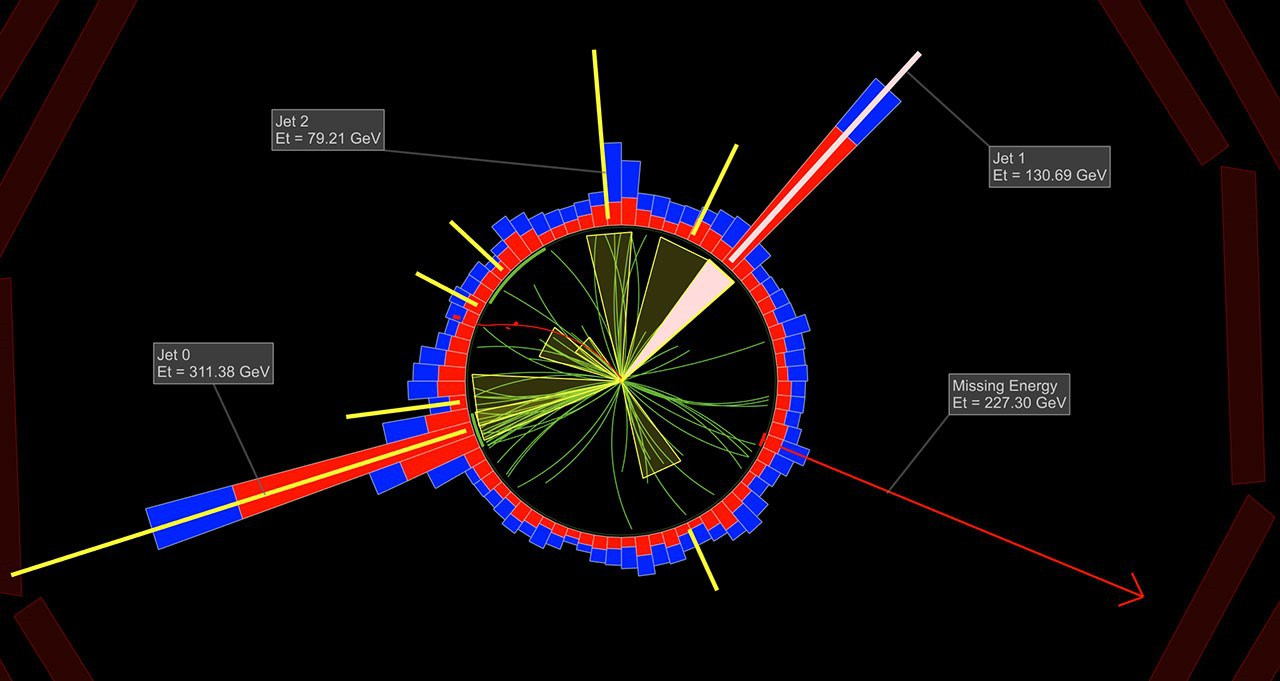
\includegraphics[width=0.95\textwidth]{collider_detection_cms}
	\caption{An image of a potential WIMP event in the CMS detector at CERN.  If a WIMP is present in a collision, momentum would not be conserved after all jets and particles have been accounted for in the collision.  Here we can see that after the three jets are reconstructed that there is still a large MET that could potentially be attributed to a WIMP.  Image courtesy: Matevz Tadel, UC San Diego/CMS.}
	\label{fig:collider_detection}
\end{figure}

One important note is that while we can potentially ``see" WIMPs in detectors at colliders,  it is impossible to be certain that this WIMP is what makes up the majority of the matter in the universe.  The same signal would need to be seen in indirect and direct searches as well to make such a confirmation \cite{queiroz2016dark}.


\subsection{Direct Detection}

The most basic models describing WIMPs predict that they are most likely to interact with atomic nuclei.  This assumption, along with cosmological evidence that WIMPs are non-relativistic, surprisingly gives way to a fairly straight-forward derivation of the rate of scattering that one could expect for different nuclei assuming a given scattering cross-section and mass for the WIMP.  We will outline the derivation presented in \citeref{lewin1996review}. 




